\begin{figure}[H]
	\centering
	\begin{subfigure}[b]{0.3\textwidth}
		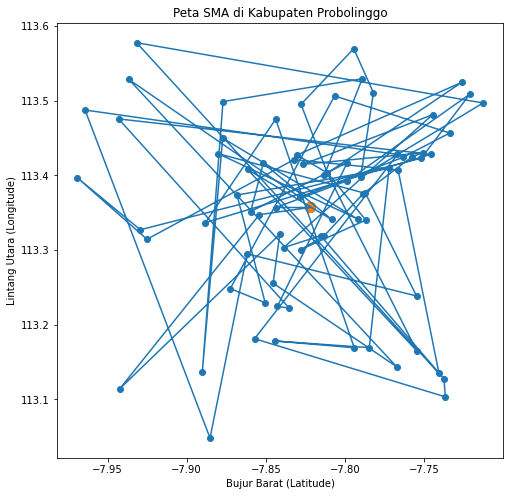
\includegraphics[width=\textwidth]{Gambar/Klaster/1.png}
		\caption{1 klaster}	
	\end{subfigure}
	\hfill
	\begin{subfigure}[b]{0.3\textwidth}
		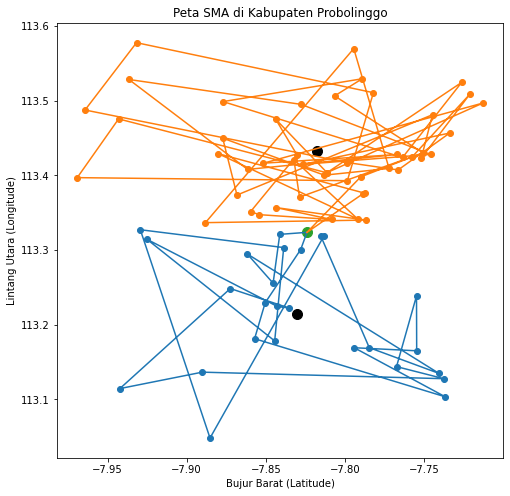
\includegraphics[width=\textwidth]{Gambar/Klaster/2.png}
		\caption{2 klaster}	
	\end{subfigure}
	\hfill
	\begin{subfigure}[b]{0.3\textwidth}
		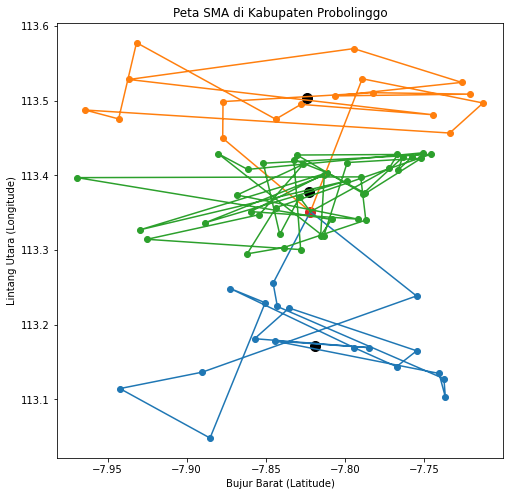
\includegraphics[width=\textwidth]{Gambar/Klaster/3.png}
		\caption{3 klaster}	
	\end{subfigure}
	\hfill
	\begin{subfigure}[b]{0.3\textwidth}
		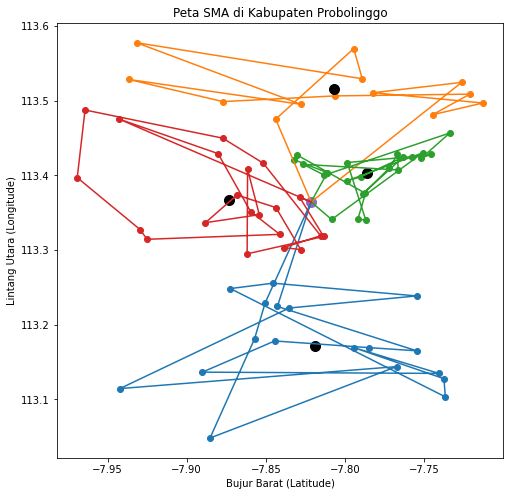
\includegraphics[width=\textwidth]{Gambar/Klaster/4.png}
		\caption{4 klaster}	
	\end{subfigure}
	\hfill
	\begin{subfigure}[b]{0.3\textwidth}
		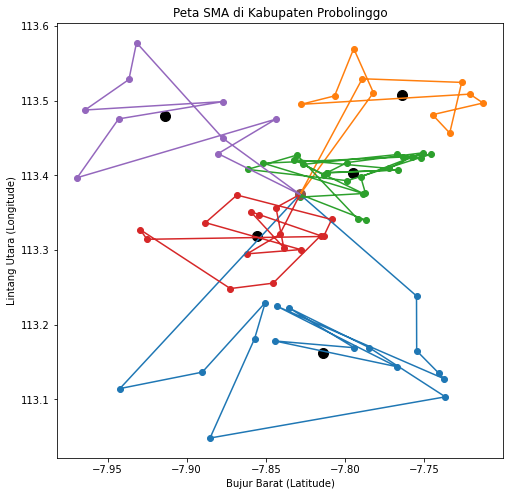
\includegraphics[width=\textwidth]{Gambar/Klaster/5.png}
		\caption{5 klaster}	
	\end{subfigure}
	\hfill
	\begin{subfigure}[b]{0.3\textwidth}
		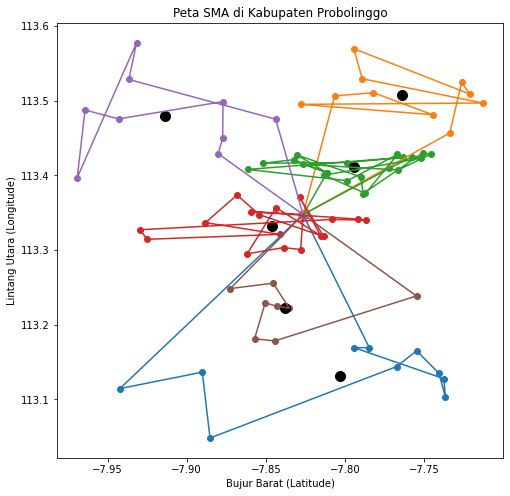
\includegraphics[width=\textwidth]{Gambar/Klaster/6.png}
		\caption{6 klaster}	
	\end{subfigure}
	\hfill
	\begin{subfigure}[b]{0.3\textwidth}
		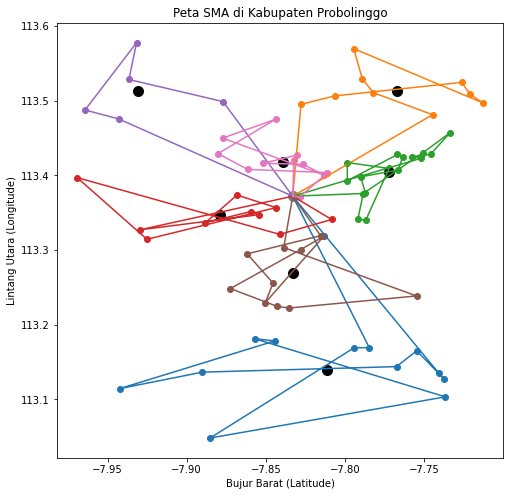
\includegraphics[width=\textwidth]{Gambar/Klaster/7.png}
		\caption{7 klaster}	
	\end{subfigure}
	\hfill
	\begin{subfigure}[b]{0.3\textwidth}
		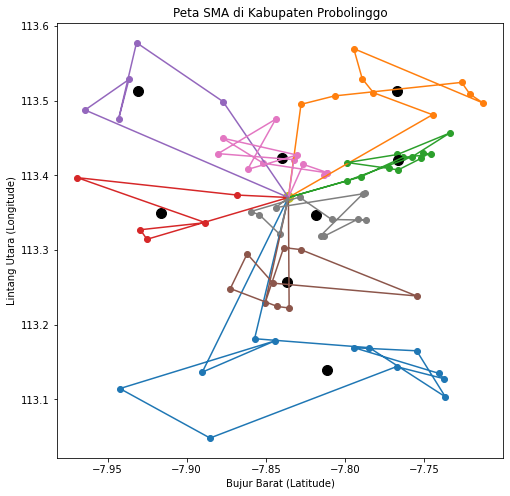
\includegraphics[width=\textwidth]{Gambar/Klaster/8.png}
		\caption{8 klaster}	
	\end{subfigure}
	\hfill
	\begin{subfigure}[b]{0.3\textwidth}
		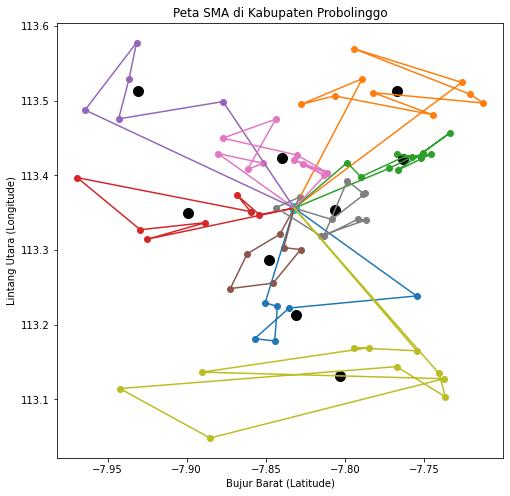
\includegraphics[width=\textwidth]{Gambar/Klaster/9.png}
		\caption{9 klaster}	
	\end{subfigure}
	\hfill
	\begin{subfigure}[b]{0.3\textwidth}
		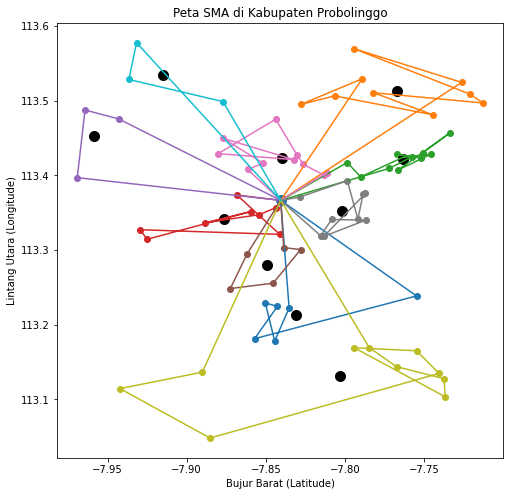
\includegraphics[width=\textwidth]{Gambar/Klaster/10.png}
		\caption{10 klaster}	
	\end{subfigure}
	\caption{Hasil rute dengan pembagian klaster berbeda}
	\label{fig:klasterbeda}
\end{figure}